% detailed  presentation of a model, including justifications for design decisions

Figure \ref{fig:MultilevelArchitecture} shows the overview of the multivel architecture designed to capture the two use cases described in the Process Challenge.

% Expliquer que le use case XSure ne nécessitait pas l'extension de metamodèle requise pour le usecase Acme Software Developement Process

\subsection{Base metamodel for the Process Challenge}

\begin{figure*}
 \centering
    % 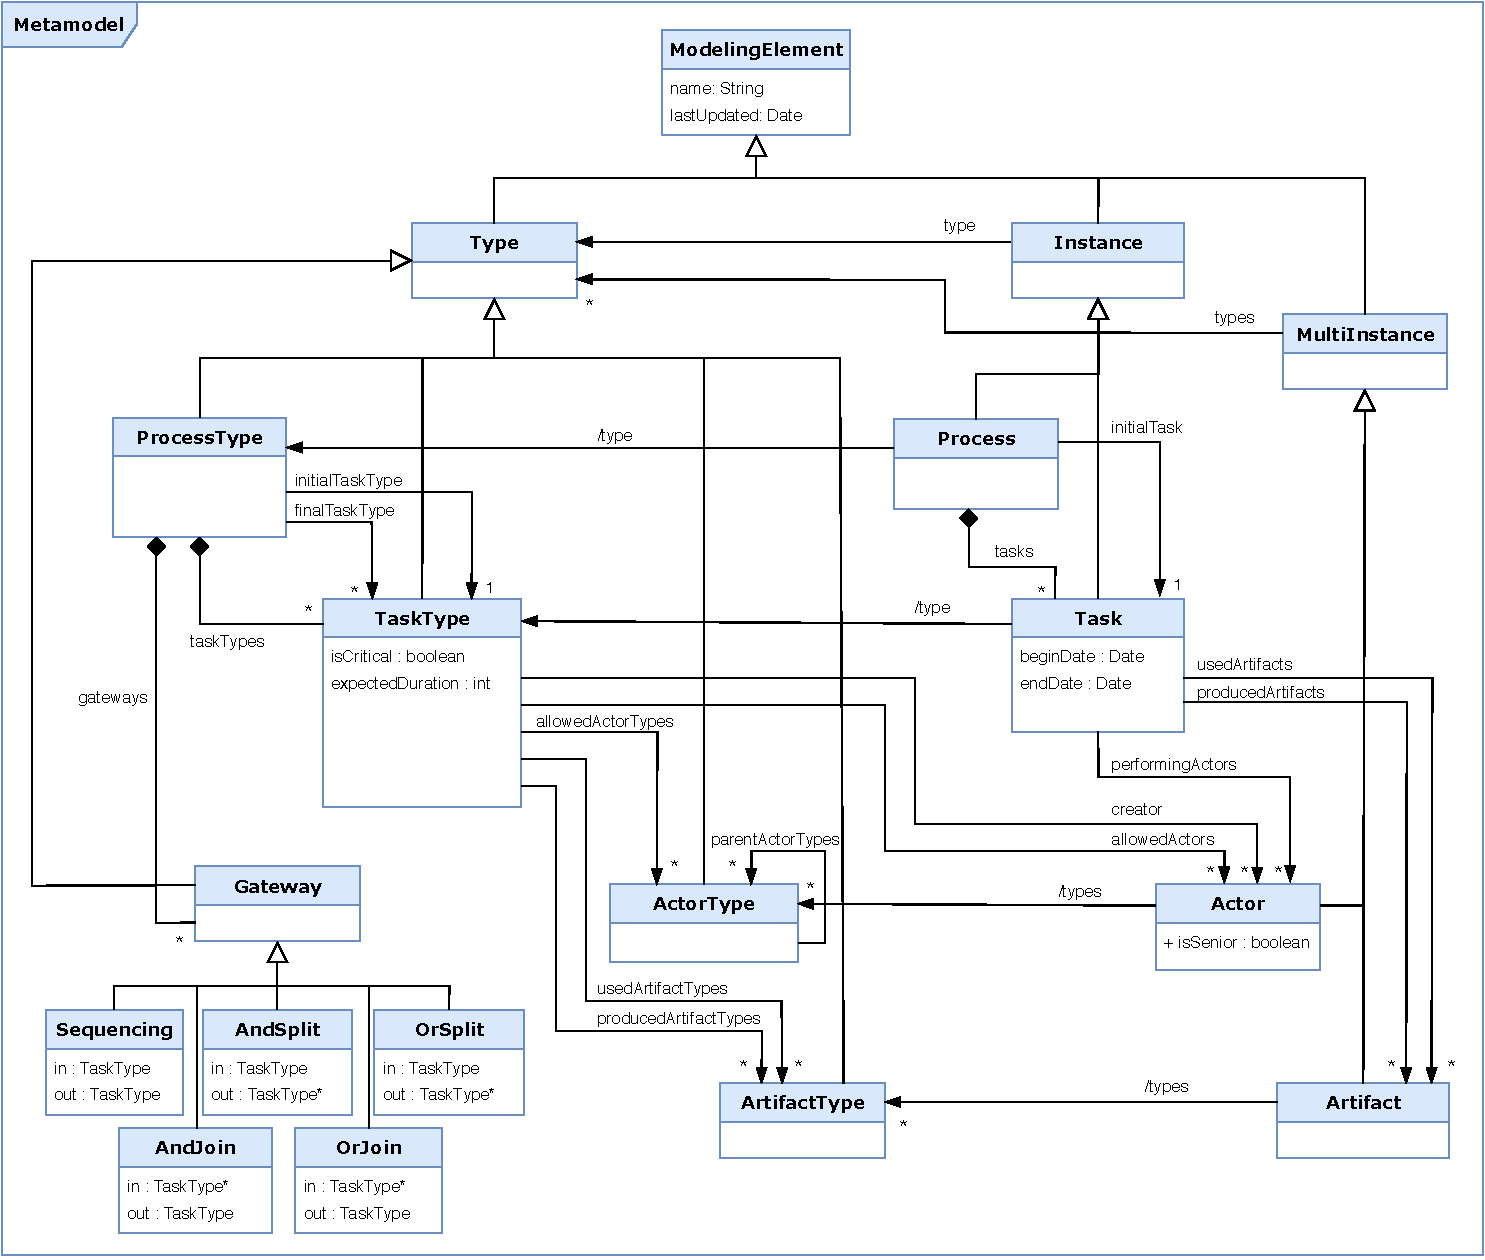
\includegraphics[width=1.0 \columnwidth]{Figures/Metamodel.pdf}
    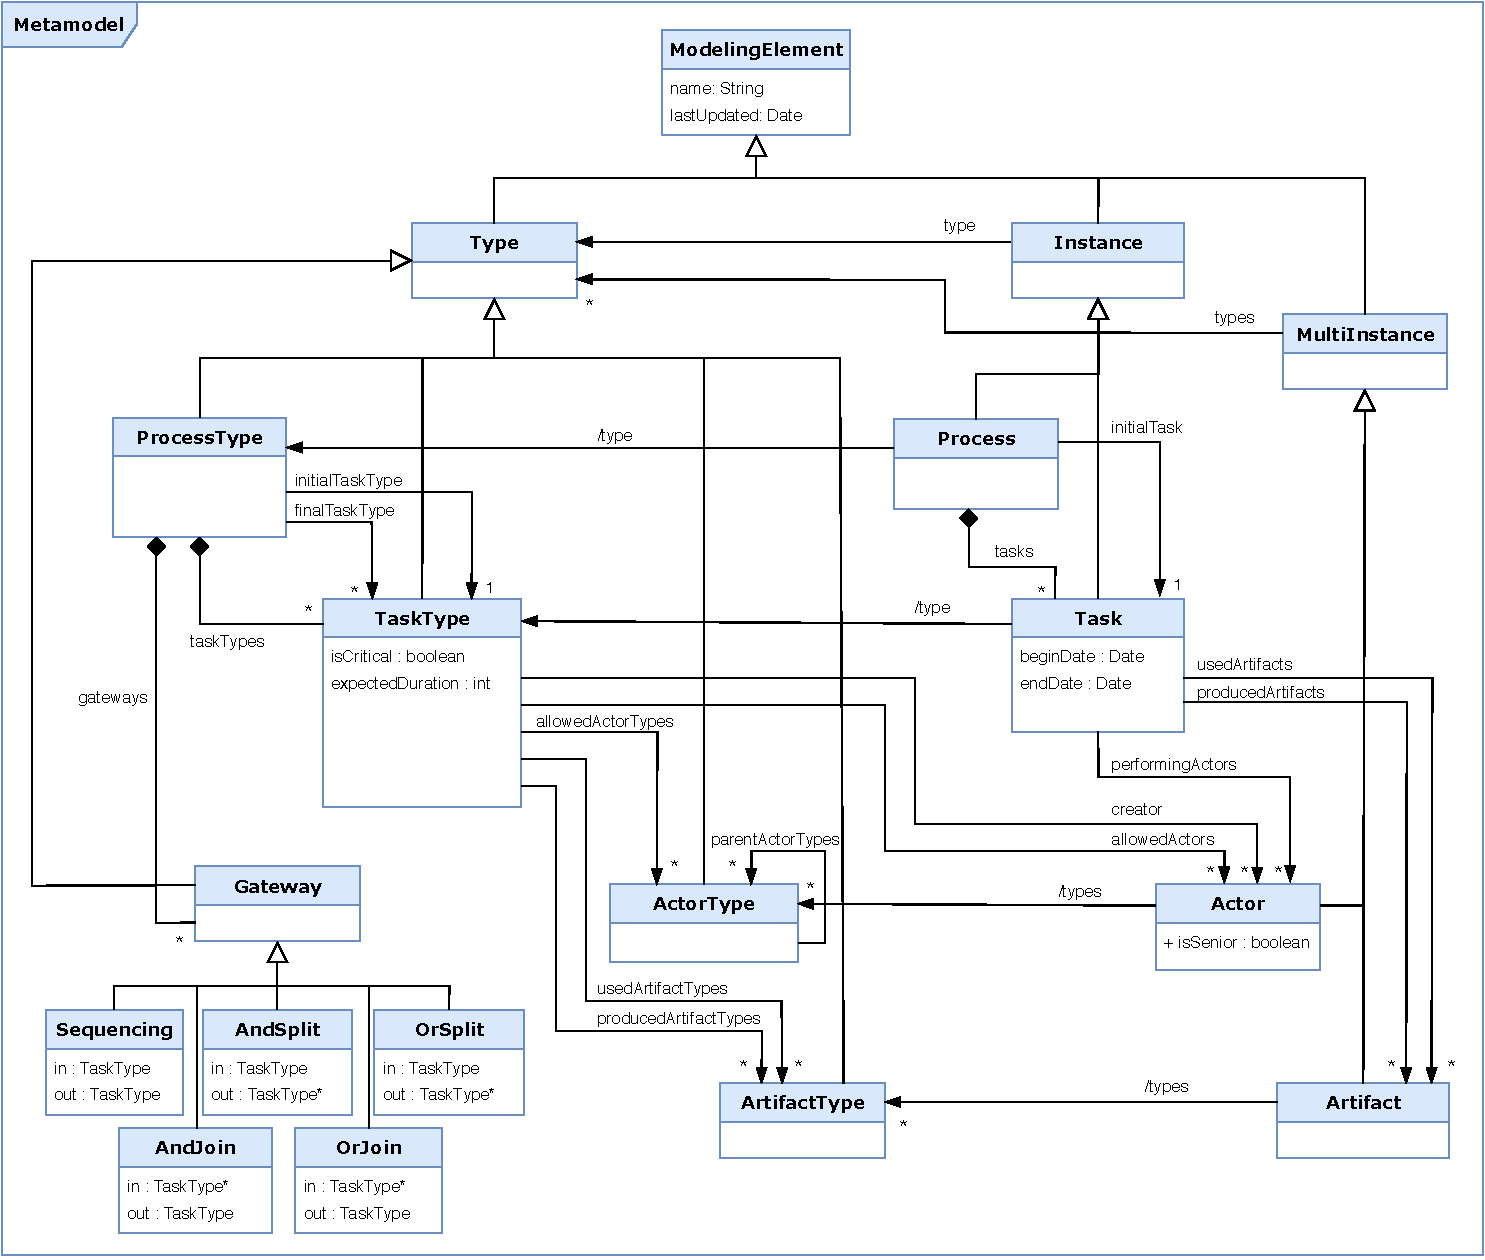
\includegraphics[width=1.0 \textwidth]{Figures/Metamodel.pdf}
     \caption{Process management base metamodel}
    \label{fig:BaseMetamodel}
\end{figure*}

In this section, we present and illustrate the base metamodel presented in figure \ref{fig:BaseMetamodel} with \textit{XSure} insurance domain use case, whose a partial description was provided in the challenge description. Note that the capture of the requirements \textbf{P1} to \textbf{P19} in the context of XSure insurance domain are straightforward implementable while instantiating \textit{XSure model}, as an instance of base metamodel (the left side of figure \ref{fig:MultilevelArchitecture}).

Figure \ref{fig:BaseMetamodel} represents this base metamodel with a UML-like formalism, well adapted to represent object-oriented FML concepts and their instances. Base conceptual element is called a \textit{FlexoConcept} in FML language, and is similar to the concept of class in object-oriented modeling. We use the UML representation of class to represent a \textit{FlexoConcept}, while cardinalities are shown using the UML-like classical rules.

Our proposition relies on ontologic instantiation as presented in figure \ref{fig:LinguisticAndOntologicInstantiation}, with a common root concept \textit{ModelingElement}. Two types of ontological instantiation are needed to meet the requirements of the challenge. One provides that some instances conform to only one type (\textit{Process} and \textit{Task} do respectively conform to one \textit{ProcessType} and \textit{TaskType}) while some entities define their conformity to several types (\textit{Actor} and \textit{Artifact} do respectively conform to several \textit{ActorType} and \textit{ArtifactType}). This instantiation is reified with the relations \textit{type} and \textit{types} between \textit{Type}, \textit{Instance} and \textit{MultiInstance} concepts.  

\subsubsection{Process type definition}

We first present the process definition part of base metamodel, located left of figure \ref{fig:BaseMetamodel}.

% Illustrer avec des instances de XSure

\textit{ProcessType} is defined as a specialization of \textit{Type} \texttt{FlexoConcept}, and references a collection of \textit{TaskType} through the composition relation \textit{taskTypes} with (0..*) cardinality (\textbf{P1}). A \textit{TaskType} is embedded in a \textit{ProcessType} and inherits from it context. To illustrate this in \textit{XSure} insurance domain use case, \textit{XSure model} defines \textit{Claim Handling}, instance of \textit{ProcessType}, and \textit{Receive Claim}, \textit{Asses Claim} and \textit{Pay premium}, instances of \textit{TaskType}.

\textit{ProcessType} also references a collection of gateways, reified with the \textit{Gateway} concept hierarchy. \textit{Gateway} is defined as a specialization of \textit{Type} and is specialized with \textit{Sequencing}, \textit{AndSplit}, \textit{AndJoin}, \textit{OrSplit} and \textit{OrJoin} concepts (\textbf{P2}). Depending of its type, a \textit{Gateway} defines one or more inputs and one or more outputs, depending of its underlying execution semantics. A \textit{ProcessType} additionally exposes unique initial \textit{TaskType} and a collection of final \textit{TaskType} with both attributes \textit{initialTaskType} (single cardinality) and \textit{finalTaskType} (cardinality 0..*) (\textbf{P3}). TaskType exposes a creator attribute as an association relation to \textit{Actor} concept (\textbf{P4}), which is in the same conceptual level. 

Following listing shows an excerpt of FML code modeling some core concepts of process modeling base metamodel. 

\begin{lstlisting}[breaklines=true, language=java, basicstyle=\ttfamily\scriptsize, mathescape=true]
model MetaModel {

  concept ModelingElement {
    ...
  }
  
  concept Type extends ModelingElement {
    ...
  }
  
  concept ProcessType extends Type {
    TaskType[0..*] taskTypes;
    TaskType initialTaskType;
    TaskType[0..*] finalTaskTypes;
    Gateway[0..*] gateways;
        
    concept TaskType extends Type {
      Actor creator;
      Actor[0..*] allowedActors;
      ActorType[0..*] allowedActorTypes;
      ...
    }
        
    abstract concept Gateway extends Type {
      abstract void executeGateway(Process process);
      ...
    }
        
    concept Sequencing extends Gateway {
      TaskType in;
      TaskType out;
    }
    
    // Other core concepts
    ...
  }
}    
\end{lstlisting}


\textit{ActorType} is defined as a sub-concept of \textit{Type} and the \textit{allowedActorTypes} relation to \textit{ActorType} which is defined in \textit{TaskType} (with 0..* cardinality) captures \textbf{P5} requirement. Requirement \textbf{P6} is symmetrically satisfied with \textit{allowedActors} relation to \textit{Actor} also defined in \textit{TaskType} (with same 0..* cardinality). Same modeling pattern applies for \textit{ArtefactType} defined as a sub-concept of \textit{Type}, and both relations \textit{usedArtifactTypes} and \textit{producedArtifactTypes} defined in \textit{TaskType} (\textbf{P7}). \textit{TaskType} additionnaly exposes an \textit{expectedDuration} attribute (expressed in number of days), satisfying \textbf{P8}. 

Actor concept defines a boolean attribute called \textit{isSenior}, while \textit{TaskType} defines an additional \textit{isCritical} boolean attribute, indicating that some instance of \textit{TaskType} are flagged as critical and must be performed by senior actors. To fullfill \textbf{P9} requirement, a supplementary constraint is required for \textit{TaskType} and is captured through this invariant expressed in FML language:

\begin{lstlisting}[breaklines=true, language=java, basicstyle=\ttfamily\scriptsize, mathescape=true]
forEach (actor : allowedActors) {
    assert !isCritical | actor.isSenior
}
\end{lstlisting}

This invariant should be completed with additional constraints defined in \textit{Task} \textit{FlexoConcept}, which apply to performing actors actually assigned to enacted tasks. 

\subsubsection{Process enactment}
\label{sec:ProcessEnactment}
We now present the process enactment part of base metamodel, located right of figure \ref{fig:BaseMetamodel}. All concepts defined in this subsection are either specialization of \textit{Instance} concept (if they are associated with exactly one \textit{Type}) or \textit{MultiInstance} concept (for those which have several types).

\textit{Process} represents an enacted \textit{ProcessType}, as defined in previous subsection (\textbf{P10}). FML defines behavioural features (operations in object-oriented modelling), called \texttt{FlexoBehaviour}. \textit{ProcessType} defines following behaviour \texttt{newProcess(String)}, taking a \texttt{String} argument (the name of the process to enact):

\begin{lstlisting}[breaklines=true, language=java, basicstyle=\ttfamily\scriptsize, mathescape=true]
public Process newProcess(String name) {    
  Process newProcess = new Process(name,this);  
  for (taskType : taskTypes) {      
    Task newTask = taskType.newTask(newProcess.name+"-"+taskType.name),newProcess);        
  }      
  return newProcess;    
}    
\end{lstlisting}

This scheme allows to rely on FML dynamic binding mechanism to delegate to types the responsability for instances creation. An instance of \textit{Process} references a unique \textit{ProcessType} trough the specialized \textit{/type} relation. Each instance of \textit{TaskType} is ontologically instantiated with a \textit{Task} (\textbf{P11}), using the same pattern where \textit{TaskType} has the responsability to manage this ontological instantiation. A \textit{Task} references its unique \textit{TaskType}, and defines a \textit{begin date} and an \textit{end date} as basic attributes of the concept (\textbf{P12}).

Same pattern applies for artifacts used and produced with relations \textit{usedArtifacts}, \textit{producedArtifacts} and \textit{performingActors} defined in \textit{Task} concept (\textbf{P13}). An instance of \textit{Artifact}, defined as a specialization of \textit{MultiInstance} concept, references a set of \textit{ArtifactType} through the specialized \textit{/types} relation (\textbf{P14} and \textbf{P16}). Likewise, concept \textit{Actor} is defined as a specialization of \textit{MultiInstance} concept and references a set of \textit{ActorType} through the specialized \textit{/types} relation (\textbf{P15}).

Authorization for an actor to perform a task (\textbf{P17}) is captured either through the relations \textit{allowedActors} and \textit{allowedActorTypes} defined in \textit{TaskType}. This mechanism is completed by following behaviours \textit{isAuthorizedActor(Actor)}, \textit{isValidActor(Actor)} and \textit{isValidActorType(ActorType)} defined in \textit{TaskType} : 

\begin{lstlisting}[breaklines=true, language=java, basicstyle=\ttfamily\scriptsize, mathescape=true]
concept TaskType extends Type {
 ...
 // Check that an Actor is authorized to perform a task, according to allowed Actor and ActorTypes
 boolean isAuthorizedActor(Actor actor) {      
  for (actType : allowedActorTypes) {        
   if (actor.hasActorType(actType))         
    return this.isValidActorType(actType);          
  }        
  for (act : allowedActors) {        
   if (actor == act)         
    return this.isValidActor(actor);          
   return false;      
 }
  
 // Check that an Actor may perform this TaskType (override when required)
 boolean isValidActor(Actor actor) {
  return true;
 }

 // Check that an ActorType may perform this TaskType (override when required)
 boolean isValidActorType(ActorType actorType) {
  return true;
 }
 ...
}
\end{lstlisting}

\textit{Task} concept basically delegates this authorization to its related \textit{TaskType}, as shown in following FML excerpt:

\begin{lstlisting}[breaklines=true, language=java, basicstyle=\ttfamily\scriptsize, mathescape=true]
concept Task extends Instance {
 ...
 boolean isAuthorizedActor(Actor actor) {      
  return type.isAuthorizedActor(actor);      
 }  
 ...
}
\end{lstlisting}

Enforcing those constraints is finally performed by the definition of this invariant in \textit{Task} concept:

\begin{lstlisting}[breaklines=true, language=java, basicstyle=\ttfamily\scriptsize, mathescape=true]
forEach (actor : performingActors) {
    assert isAuthorizedActor(actor);
}
\end{lstlisting}

Default behaviour states that all actors and actor types are valid for all task types. This modelling scheme offers many extension points, by the redefinition of one or some behaviours in inherited concepts (although none were required in the context of XSure insurance use case).

Actor types specialization is captured by the \textit{parentActorTypes} relation defined in \textit{ActorType} (\textbf{P18}). This is completed by both the definition of \textit{hasActorType(ActorType)} behaviour in \textit{Actor} concept and recursive behaviour \textit{isOrSpecializes(ActorType)} in \textit{ActorType}:

\begin{lstlisting}[breaklines=true, language=java, basicstyle=\ttfamily\scriptsize, mathescape=true]
concept ActorType extends Type {
 ActorType[0..*] parentActorTypes;
 ...
 boolean isOrSpecializes(ActorType actorType) {    
  if (actorType = this)   
   return true;      
  for (p : parentActorTypes) {      
   if (p.isOrSpecializes(actorType)
    return true;        
  return false;    
 }
 ...
}

concept Actor extends MultiInstance {
 ...
 boolean hasActorType(ActorType actType) {      
  for (type : types) {
   if (type.isOrSpecializes(actType)) {
    return true;
   }
  }     
 }  
 ...
}
\end{lstlisting}

All concepts inherits from \textit{ModelingElement}, which defines a \textit{lastUpdated} attribute with \textit{Date} type, and thus satisfies \textbf{P19} requirement. 

\subsection{The Acme software development process}
\label{sec:AcmeSoftwareDevelopmentProcess}

The challenge describes in a second part a Software engineering process for a fictional Acme company. Base metamodel as described in previous section is too generic to capture all domain-specific aspects of this use case. We choose to complete the architectual hierarchy with a specific metamodel, specific to Acme software development process, as shown in figure \ref{fig:AcmeArchitecture}. \textit{Acme metamodel} inherits and specializes base metamodel, and \textit{Acme model} is defined as an instance of \textit{Acme metamodel}. Any instance of Acme model is either an instance of a concept defined in base metamodel, or a concept defined in specialized Acme metamodel, which may or not inherit from a concept defined in base metamodel.
% FML follows a classical object-oriented semantics. ???

\begin{figure}
 \centering
    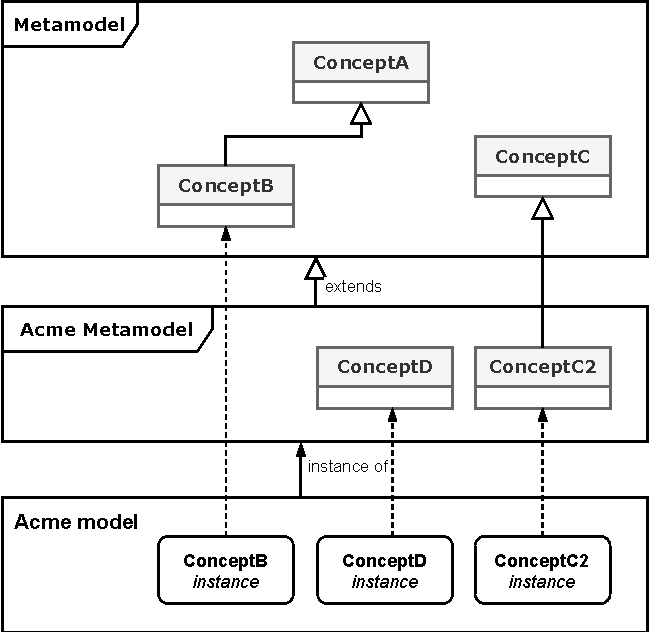
\includegraphics[width=1.0 \columnwidth]{Figures/AcmeArchitecture.pdf}
     \caption{Acme software development process architecture}
    \label{fig:AcmeArchitecture}
\end{figure}

\begin{figure*}
 \centering
     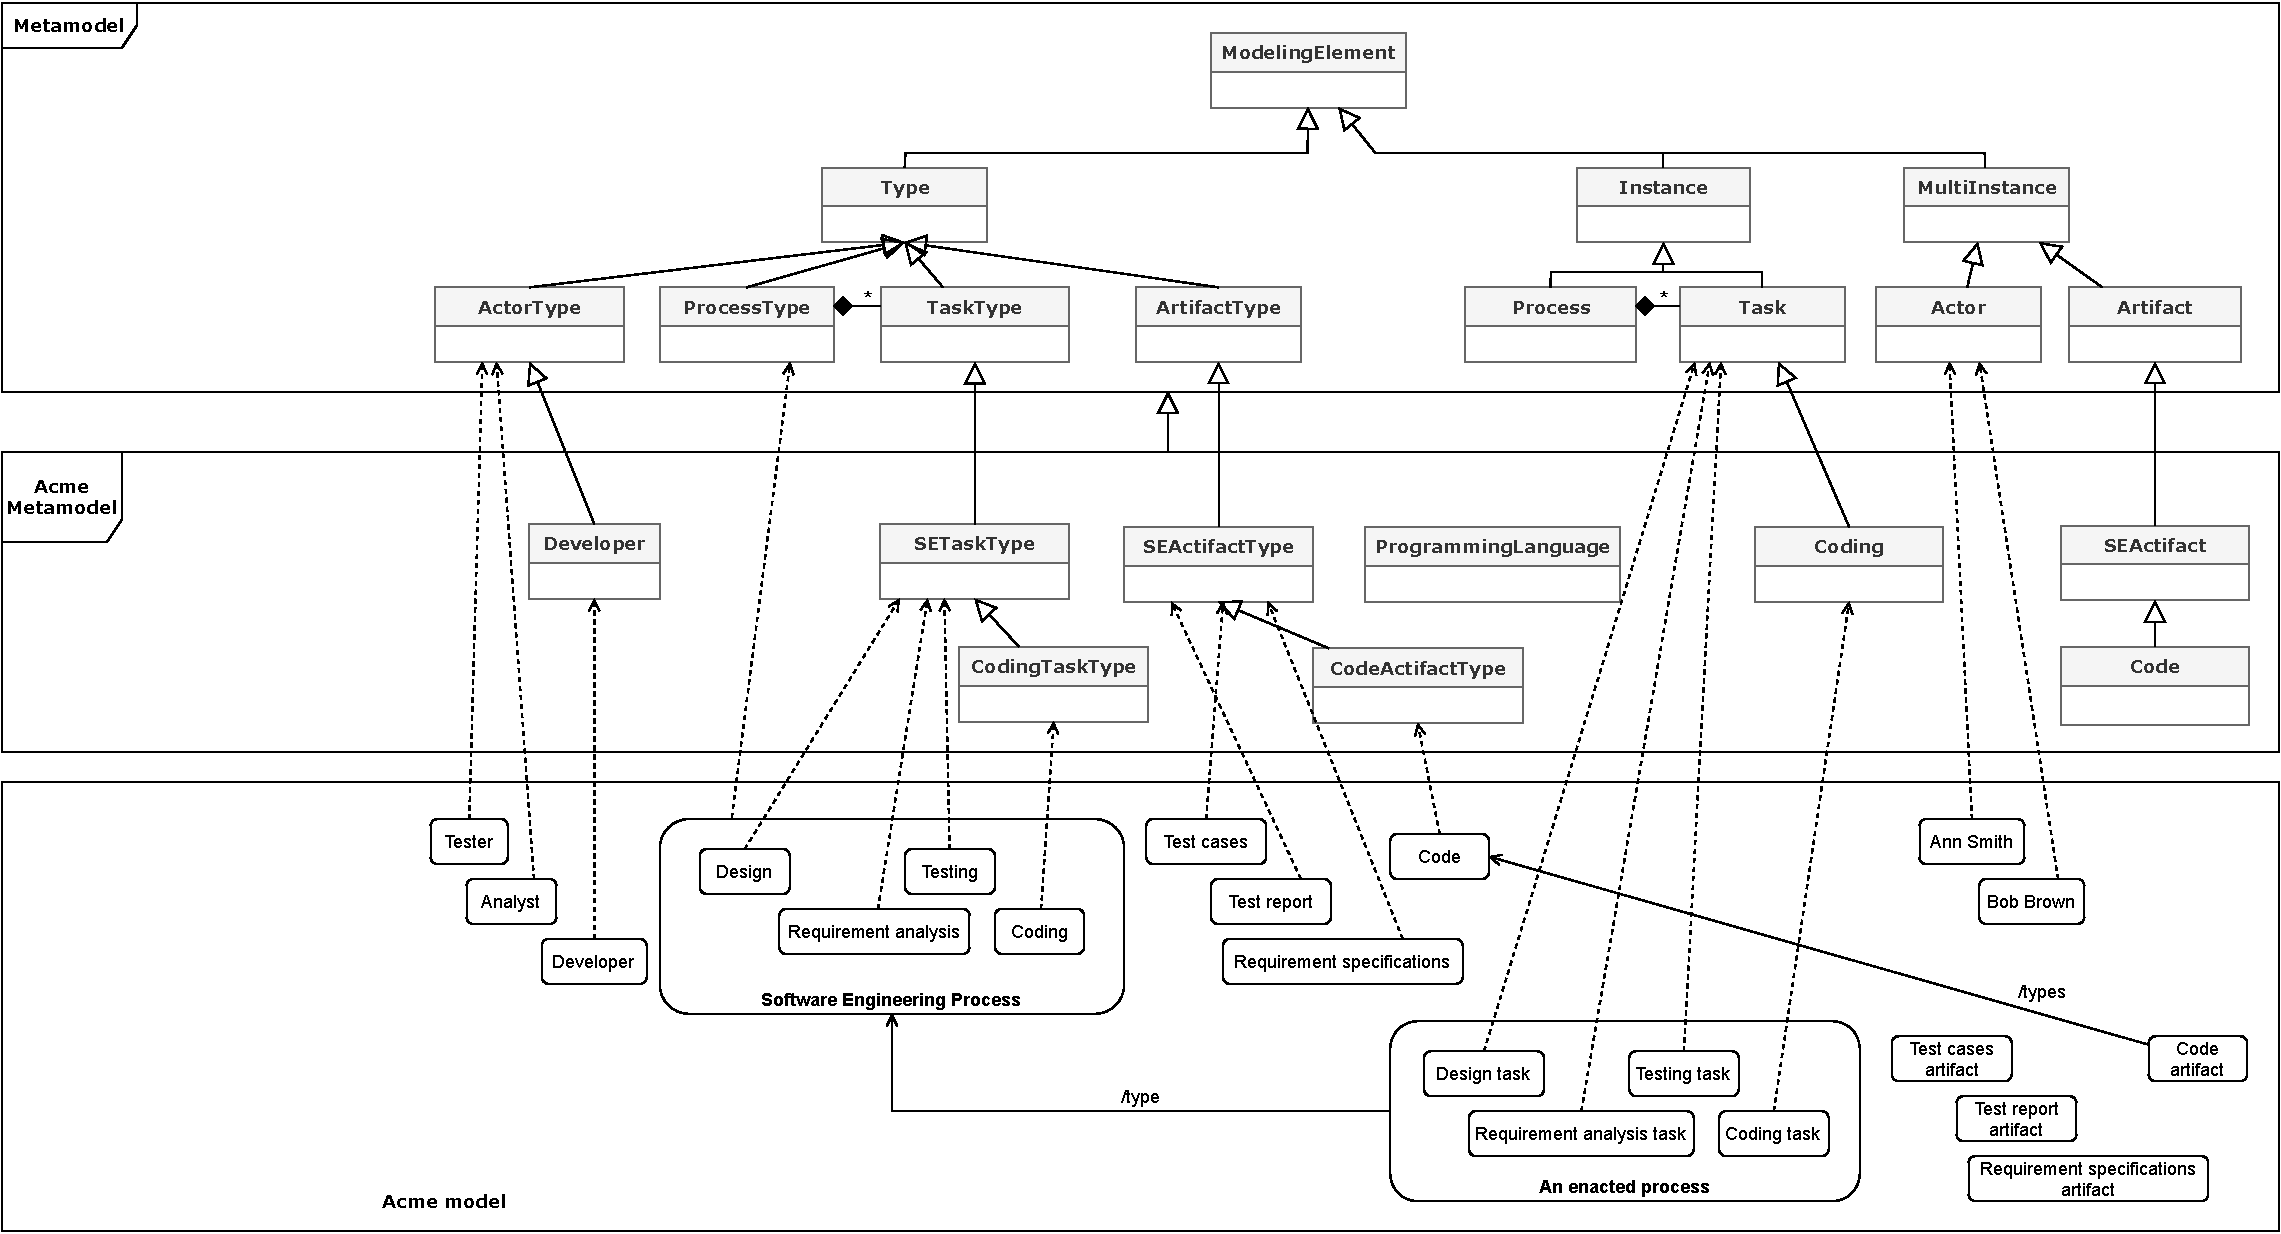
\includegraphics[width=1.0 \textwidth]{Figures/AcmeFullArchitecture.pdf}
     \caption{Acme software development process architecture}
    \label{fig:AcmeFullArchitecture}
\end{figure*}




\subsection{Openflexo tooling}

% Expliquer l'outillage construit et comment il marche


